% Beamer is used as a portrait reading-document layout, not a slide deck.
% This also permits an offline build with the cluster's existing TeX cache.
\documentclass[12pt]{beamer}
\geometry{paperwidth=8.5in,paperheight=11in}
\setbeamersize{text margin left=0.85in,text margin right=0.85in}
\setbeamertemplate{navigation symbols}{}
\setbeamertemplate{footline}{\hfill\small\insertframenumber\hspace{0.85in}\vspace{0.4in}}
\usepackage[T1]{fontenc}
\usepackage{lmodern}
\usepackage{amsmath,amssymb,booktabs,array}
\usepackage{xcolor}
\usepackage{tikz}
\usetikzlibrary{arrows.meta,positioning}
\definecolor{ink}{HTML}{18354B}
\definecolor{wash}{HTML}{EDF3F7}
\definecolor{accent}{HTML}{267D72}
\setlength{\parindent}{0pt}
\setlength{\parskip}{7pt}
\setlength{\emergencystretch}{2em}
\newcommand{\takeaway}[1]{\par\medskip\noindent\colorbox{wash}{\parbox{\dimexpr\linewidth-2\fboxsep\relax}{\textbf{The main idea.} #1}}\par\medskip}
\newcommand{\chapterpage}[2]{{\small\color{accent}\textbf{#1}}\par{\LARGE\color{ink}\textbf{#2}}\par\medskip}
\newcommand{\question}[1]{\par\smallskip{\large\color{ink}\textbf{#1}}\par}
\hypersetup{pdftitle={Learning RL by reproducing CURL},pdfauthor={RLM research notebook},colorlinks=true,urlcolor=blue!55!black,linkcolor=blue!55!black}
\begin{document}
\begin{frame}[t]
\vspace*{0.55in}
{\small\color{accent}\textbf{REPRODUCTION NOTEBOOK \quad | \quad 7 OCTOBER 2026}}

{\huge\color{ink}\textbf{Learning reinforcement learning\\by reproducing CURL}}

{\large A guide to the experiment, the code, and the evidence we need.}

\takeaway{We want a small training experiment whose behavior we can explain and check. First we will reproduce an existing method. Then we will remove one component to ask what it contributes.}

\question{Where are we now?}

\textbf{CURL finished higher in the original three short cartpole comparisons.}
After five times as much training, its average advantage became much smaller,
with different winners across runs. This is an early benefit in a small study,
not proof of a lasting advantage or equivalence. Pages 8--9 show every pair.

Walking results varied more: both training groups had different winners.
Their average scores were \textbf{435 versus 433} and \textbf{398 versus 231}
(CURL first). Pages 10--12 keep both groups visible. New test starts did not
change the original pair-by-pair winners.

Wrong image matches hurt cartpole learning in every tested seed. Reducing the
matching update did not remove that harm. With correct matches, the smaller
update has not shown a dependable improvement. Pages 13--14 show the original
comparison. \textbf{All nine fresh-seed models have now finished: both matching
methods won twice and lost once against no matching.} Averages hide large
differences between runs. Page 15 shows the complete new group and what it
changes. Results finished on 5 October; reviewed on 7 October, 08:45 UTC.

\question{Why this paper?}

CURL combines two kinds of learning in a compact setting: learning which actions
earn reward, and learning useful visual features by matching related images.
The authors provide code. This gives us concrete pieces to inspect and compare
without starting with a large language-model training system. The paper is
\emph{CURL: Contrastive Unsupervised Representations for Reinforcement Learning},
by Laskin, Srinivas and Abbeel, ICML 2020.\footnote{\url{https://proceedings.mlr.press/v119/laskin20a.html}}

\question{What this exercise does not cover}

This is not an RLM and does not train a language model. It does not use
supervised fine-tuning (SFT), where a model imitates supplied answers or actions.
Here, self-supervised learning (SSL) means constructing an image-matching task
from the agent's own observations. Reinforcement learning (RL) uses rewards
from a simulator. A successful reproduction would improve our experimental
practice, but would not retroactively prove our earlier RLM training correct.

\question{How to read this guide}

Pages 2--4 explain the task with examples. Pages 5--6 explain the comparison
and code. Pages 7--15 give next decisions, checks and measured results.
Teaching examples are labeled; published reference scores belong to the authors.

\end{frame}
\begin{frame}[t]
\vspace*{0.55in}
\chapterpage{1 / THE TASK}{What does the model actually do?}

Imagine a cart that moves left and right on a track. A pole is attached to the
cart. The controller must move the cart to swing the pole upward and keep it
balanced. We use the \texttt{cartpole/swingup} task from DeepMind Control Suite,
not the similarly named Gym CartPole benchmark.

\begin{center}
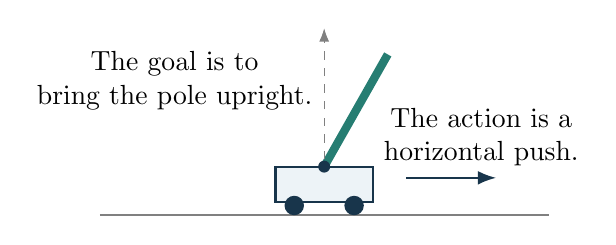
\begin{tikzpicture}[>=Latex,scale=0.95]
  \draw[thick,gray] (-3,0)--(3,0);
  \filldraw[fill=wash,draw=ink,thick] (-.65,.18) rectangle (.65,.65);
  \fill[ink] (-.4,.13) circle (.13); \fill[ink] (.4,.13) circle (.13);
  \draw[line width=3pt,accent] (0,.65)--(.85,2.15);
  \fill[ink] (0,.65) circle (.08);
  \draw[->,thick,ink] (1.1,.5)--(2.3,.5);
  \node[align=center] at (2.1,1.05) {The action is a\\horizontal push.};
  \draw[->,dashed,gray] (0,.75)--(0,2.5);
  \node[align=center] at (-2,1.8) {The goal is to\\bring the pole upright.};
\end{tikzpicture}

{\small Conceptual drawing, not an observation from a local simulator run.}
\end{center}

\question{The input is pictures, not the correct action.}

The learner receives three recent color images together. Several images help
it distinguish a pole moving left from one moving right, even when one snapshot
looks similar. It is not handed the pole's angle and velocity as the policy's
input. A neural network first turns these pixels into a compact numerical
description. This part is called the \textbf{encoder}.

The \textbf{policy}, also called the actor, uses that description to choose a
continuous action: how hard to push the cart. Its weights are the numbers changed
during training. For this reproduction they start from random initialization,
not from a pretrained language model or a demonstration dataset.

\question{The simulator provides feedback.}

After a push, the simulator returns new images and a numerical reward. The task's
reward function defines which behavior is desirable. The learner does not get a
label saying, ``the correct action was to push left.'' It has to learn which
actions lead to better outcomes over time.

\takeaway{This is trial-and-error learning with feedback, not imitation of an expert's actions. The simulation supplies experiences as training proceeds.}

\question{Where is the dataset?}

The agent builds it while acting. Each record contains an observation, its
action, the resulting reward, the next observation and whether the episode
ended. Old records are kept in a \textbf{replay buffer}: a memory of experience
that can be sampled repeatedly. Evaluation episodes are kept out of that memory.

\end{frame}
\begin{frame}[t]
\vspace*{0.55in}
\chapterpage{2 / TWO LEARNING SIGNALS}{What is CURL learning from?}

The task reward teaches the controller what to accomplish. CURL adds another
exercise to help the encoder interpret its pictures. That exercise does not
require someone to label the images.

\question{A concrete image-matching example}

Take one recorded three-image observation of a pole leaning right. Make two
slightly different crops of it. Those two views come from the same observation,
so we know that they should match. Views cropped from other recorded observations
serve as alternatives. The pictures below are simplified labels, not actual frames.

\begin{center}
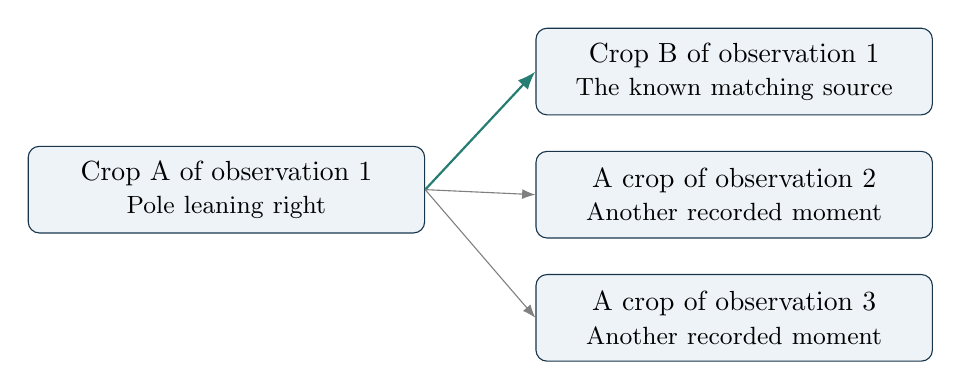
\begin{tikzpicture}[>=Latex,
  box/.style={draw=ink,rounded corners,fill=wash,align=center,text width=4.8cm,minimum height=1.1cm}]
  \node[box] (q) {Crop A of observation 1\\\small Pole leaning right};
  \node[box,right=1.4cm of q,yshift=1.5cm] (a) {Crop B of observation 1\\\small The known matching source};
  \node[box,below=.45cm of a] (b) {A crop of observation 2\\\small Another recorded moment};
  \node[box,below=.45cm of b] (c) {A crop of observation 3\\\small Another recorded moment};
  \draw[->,thick,accent] (q.east)--(a.west);
  \draw[->,gray] (q.east)--(b.west);
  \draw[->,gray] (q.east)--(c.west);
\end{tikzpicture}
\end{center}

The matching target comes from how we constructed the pair. It is not an expert
action and not the task reward. This is the \textbf{self-supervised} part. The
method is \textbf{contrastive} because it compares a known match with alternatives.
Different observations can still look very similar; being a different record
does not guarantee a meaningfully different physical situation.

\question{What does one loss calculation mean?}

Suppose the model assigns similarity scores 2, 0 and $-1$ to those three
candidates, with the correct match first. Taking the exponential of each score
gives positive weights of approximately 7.389, 1 and 0.368. Dividing the matching
weight by the total gives
\begin{center}
Probability of the match = 7.389 / (7.389 + 1 + 0.368)\\
which is approximately 0.844.
\end{center}
The matching loss is the negative natural logarithm of that probability,
approximately 0.170. If all three scores were equal,
the probability would be 1/3 and the loss about 1.099. Lower loss means that
this matching exercise is going better. \textbf{These are invented teaching
numbers, calculated directly, not training measurements.}

\takeaway{CURL's hope is that learning to recognize related views helps the controller learn from fewer interactions. A lower image-matching loss alone does not prove better control.}

\end{frame}
\begin{frame}[t]
\vspace*{0.55in}
\chapterpage{3 / THE TRAINING LOOP}{How do the weights get updated?}

CURL's control learner is Soft Actor-Critic (SAC). The most useful distinction
is between choosing actions and estimating their consequences. The
\textbf{actor} chooses an action. A \textbf{critic} estimates how much future
reward that action could lead to. The implementation uses two critics to reduce
reliance on an overly optimistic estimate.

\begin{center}
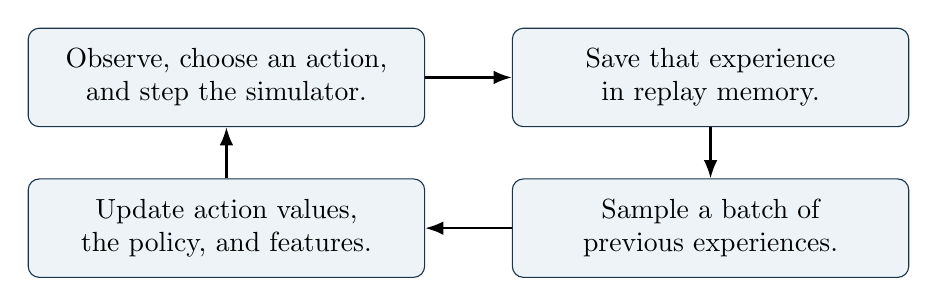
\begin{tikzpicture}[>=Latex,
  box/.style={draw=ink,rounded corners,fill=wash,align=center,text width=4.8cm,minimum height=1.25cm}]
  \node[box] (act) {Observe, choose an action,\\and step the simulator.};
  \node[box,right=1.1cm of act] (save) {Save that experience\\in replay memory.};
  \node[box,below=.65cm of save] (batch) {Sample a batch of\\previous experiences.};
  \node[box,left=1.1cm of batch] (learn) {Update action values,\\the policy, and features.};
  \draw[->,thick] (act)--(save); \draw[->,thick] (save)--(batch);
  \draw[->,thick] (batch)--(learn); \draw[->,thick] (learn)--(act);
\end{tikzpicture}
\end{center}

\question{What teaches the critic?}

For a saved transition, it compares its previous prediction with the reward
actually received plus an estimate of what can happen next. In simplified form,
\begin{center}
Target = reward now + discounted estimate of future value.
\end{center}
The discount factor gives less weight to distant rewards. SAC also includes an
exploration term and special handling of episode endings; this equation explains
the idea, not every term of the implementation.

\question{What teaches the actor and encoder?}

The actor is updated toward actions the critics value, while SAC also encourages
some action diversity. The encoder receives learning signals from predicting
values and from CURL's image-matching exercise. Related target networks change
gradually, rather than immediately copying every update. This helps prevent the
learner's targets from moving too abruptly. Exact parameter sharing and update
order matter; we preserve the authors' implementation before making changes.

\question{What does the computer do during a run?}

The CPU advances the simulation and manages experience; the GPU performs neural
network calculations. Training begins with random actions to fill replay memory.
It then alternates collection with updates. The first protocol uses 1,000 random
action decisions and batches of 128 replay records. A single GPU is sufficient
for this experiment. Our completed 100,000-step training/evaluation loops took
about 13--14.4 minutes each, excluding setup and the final checkpoint write.

\takeaway{One interaction and one gradient update are different things. Replay lets the learner revisit old experience. We must record both the amount of experience and the amount of computation.}

\end{frame}
\begin{frame}[t]
\vspace*{0.55in}
\chapterpage{4 / THE COMPARISON}{How will we know whether it worked?}

There are two questions, and they need different evidence.

\question{First: can we reproduce a published result?}

We start with the authors' CURL implementation on cartpole swing-up. The paper's
Table 1 reports the following episode returns. The spread is the standard
deviation across ten separately trained seeds, not a confidence interval.

\begin{center}
\begin{tabular}{lll}
\toprule
Training experience & Authors' CURL result & Our CURL result\\
\midrule
100,000 simulator steps & 582 (SD 146) & 571 (SD 117; 3 seeds)\\
500,000 simulator steps & 841 (SD 45) & 855 (SD 12; 3 seeds)\\
\bottomrule
\end{tabular}
\end{center}

We will report any modern software changes and use the published values as
reference points, not declare success because one lucky run enters that range.
Our three-seed summaries are smaller than the authors' ten-seed report.
The individual longer CURL scores were 843, 866 and 855. The first required
extra recovery interactions; the other two did not. This is not an equal-cost
comparison with the published experiment. Matching a published score does not
show which part of the method helped. Our matched controls answer a different
question, with their complete longer results shown on page 9.

\question{Second: does the extra matching objective help?}

Compare CURL with the same learner after removing only the contrastive update.
Keep random image crops in both arms. Otherwise, an apparent benefit could come
from cropping rather than the extra learning objective. This is our controlled
ablation, \textbf{not necessarily the paper's ``Pixel SAC'' baseline}.

\question{What do the axes and score mean?}

The plot on page 8 puts \textbf{training simulator steps} on the horizontal axis
and \textbf{mean evaluation episode return} on the vertical axis.
An episode return is the sum of its rewards. At each evaluation we average ten
episodes without changing the weights. Higher return means better performance
under this reward function, not a percentage of questions answered correctly.
It shows each training seed, not only a smoothed average.

\takeaway{The cartpole setting repeats each chosen action eight times. So 12,500 model decisions normally produce 100,000 simulator steps. Evaluation interactions are counted separately.}

We evaluate a separate simulator with fixed seeds and deterministic actions.
Ten episodes of one trained policy tell us about that policy; they are not ten
independent training runs. We compare the fixed final checkpoint, not the most
flattering point on the curve. Time and GPU use are separate measurements:
learning from less experience need not mean finishing faster.

\end{frame}
\begin{frame}[t]
\vspace*{0.55in}
\chapterpage{5 / WHAT SOURCE REVIEW FOUND}{What could make a run misleading?}

These findings concern the implementation, not which method performs better.
The review uses upstream commit \texttt{8416d6e3869e38ca0e46fcbc54a2f784dc09d7fc}.

\question{A saved model is not necessarily a resumable run.}

The training script's \texttt{--save\_model} path saves CURL's representation
module. That does not include the full acting policy and learning state. Another
method saves actor and critic weights, but still omits important state.

For resumption, we also need optimizer history, target networks, the learned
exploration parameter, replay memory, counters and random-generator states.
To continue the same trajectory, we need simulator state and recent frames too.
Restarting at a new episode can be useful, but must not be described as an
identical continuation. Our CPU test restored the actual upstream agent and
reproduced its next fixed-batch update exactly, including shared parameters.

A longer run also exposed a defect in \emph{our} saving code: one replay array
grew beyond the old format's size limit. The previous checkpoint survived.
We changed the format and tested saving and reloading an array larger than
4 GiB. Small pilot tests had not exercised this limit.

\question{Evaluation should not disturb the training world.}

The upstream loop evaluates using the same environment object used for training.
If evaluation resets that object halfway through a training episode, the stored
observation can stop matching the simulator's actual state. We use a separate
evaluation environment and preserved training random state. This is a documented
adaptation; it is not evidence that this failure occurred in the paper's runs.

\question{The exact optimizer wiring matters.}

Two optimizers in the contrastive update include the same query encoder
parameters, and both take a step. A clean-room implementation with only one step
would therefore not automatically match this released code. Our fixed-batch
tests check this behavior, and our reference runs preserve it. Our completed
comparison removes only one of those steps deliberately. Page 14 shows its
mixed effects. This tests sensitivity to the update's strength; it is not a
correction of an established bug.

\question{A quickstart command is not the paper's protocol.}

The README's example runs one million model decisions. That is not the paper's
100,000-simulator-step comparison. The old dependencies also need a pinned
compatibility stack. We must identify changes to rendering, environment behavior
and learning code instead of assuming that a program which starts is a faithful
reproduction.

\takeaway{The lesson is not to build a huge testing system before learning anything. It is to check the few details that can change the scientific meaning of the result.}

These findings come from the authors' MIT-licensed implementation.\footnote{\url{https://github.com/MishaLaskin/curl/tree/8416d6e3869e38ca0e46fcbc54a2f784dc09d7fc}}
The hyperparameters and step terminology are documented in the supplement.\footnote{\url{https://proceedings.mlr.press/v119/laskin20a/laskin20a-supp.pdf}}

\end{frame}
\begin{frame}[t]
\vspace*{0.55in}
\chapterpage{6 / OUR NOTEBOOK}{What happens next, and what can we conclude?}

\question{The next useful sequence}

All three original cartpole pairs have completed at both 100,000 and 500,000
training steps. We continued the same saved models to ask whether the early
advantage lasts with more training. Every original model is included, regardless
of its score. Resuming a model does not create another independent training run.

The first extension stopped at 409,000 steps because saving failed. Its latest
intact state was at 307,000. After recovery it reached 500,000 and scored 843.
The repeated branch still cost 102,000 interactions: this model used 602,000
physical training interactions in total. We keep those costs and the abandoned
measurements separate from the model's retained training history.

\question{How results will change the plan}

The control finished higher in two longer cartpole pairs; CURL won one.
Both completed walking groups also have different winners, though the new group
favors CURL on average. The benefit varies across training runs. The completed
wrong-matching comparison now shows that false teaching targets can hurt
cartpole learning. That harm remained after reducing the matching update;
the smaller update did not consistently improve correct matching either.

Our independent small NumPy calculation matches the released Torch loss and
gradients to numerical precision. That checks the calculation, not its usefulness
for control. We need the matched experiment to answer the latter question.

\question{What has actually been established today?}

\begin{tabular}{p{.48\linewidth}p{.44\linewidth}}
\toprule
Item & Status\\
\midrule
Paper and core source review & Complete for the first task.\\
Budget and comparison specified & Yes; modern simulator stack recorded.\\
Training and evaluation & Cartpole, walking and wrong-match tests.\\
Checkpoint save/reload verification & Next-update and large-array tests passed.\\
Evidence about the extra matching task & Cartpole and walking: variable benefits.\\
\bottomrule
\end{tabular}

\question{What did the fresh models tell us?}

All nine fresh cartpole models finished: original CURL, smaller-update CURL
and no matching, each with three new training seeds. Both matching methods
beat no matching twice and lost once. The smaller update beat original CURL
once and lost twice, just as in the original group. Page 15 reports every
new result separately from the old group. The next useful question is why
the benefit varies, not which single run has the most favorable score.

\takeaway{Our immediate goal is a trustworthy learning example, not a novelty claim. The transferable skills are controlling comparisons, reading the actual update, evaluating fairly, and preserving enough state to explain and resume a run.}

\small
\textbf{Research records.} The configuration and execution handoff are in
\nolinkurl{experiments/curl_replication_20261004/README.md} and
\nolinkurl{experiments/curl_replication_20261004/manifest.json}.
Earlier RLM work is preserved in
\nolinkurl{docs/RESEARCH_RESUME_2026-10-04.md}.
\end{frame}
\begin{frame}[t]
\vspace*{0.55in}
\chapterpage{7 / THREE EARLY COMPARISONS}{CURL was ahead after 100,000 steps.}

At the fixed 100,000-step endpoint, CURL scored \textbf{678 versus 454} in the
first pair, \textbf{446 versus 241} in the second, and \textbf{588 versus 463}
in the third. Its control uses the same
random crops but no image-matching update. Higher reward means better swinging
and balancing, not a percentage of successful episodes.

\begin{center}
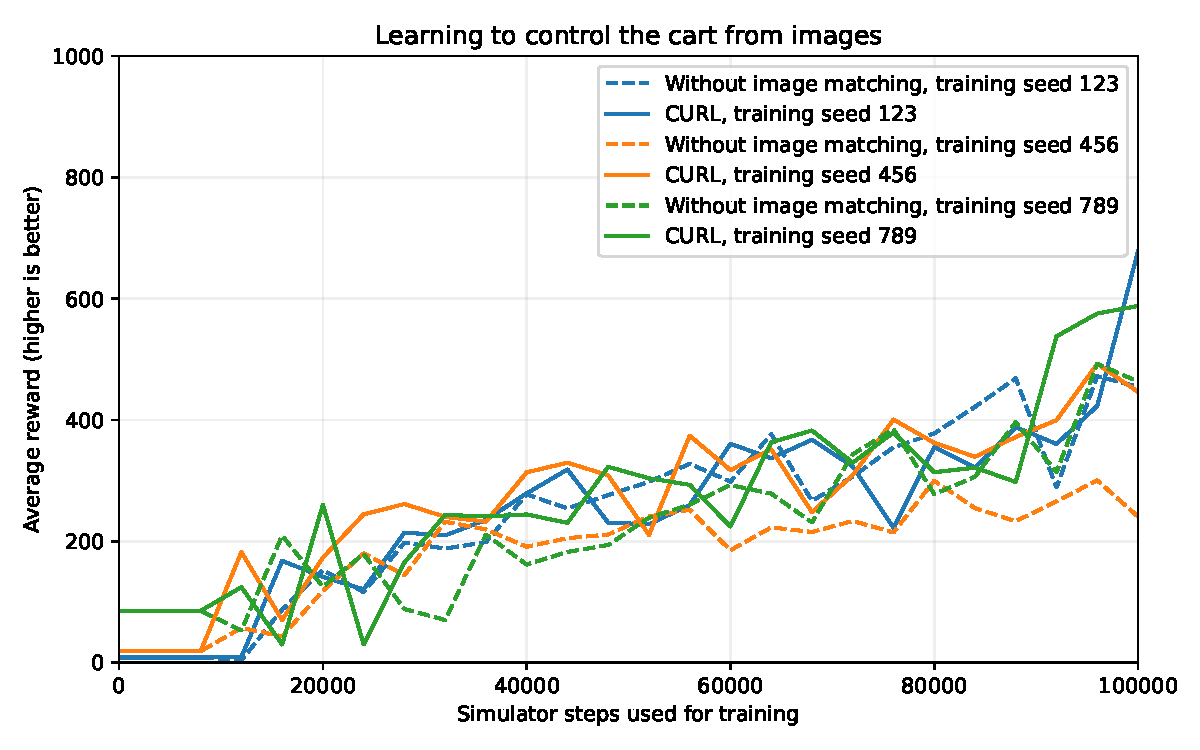
\includegraphics[width=.90\linewidth]{figures/three-pairs.pdf}
\end{center}

Solid lines are CURL; dashed lines are the control. Each color is a separate
training seed, which changes initialization and training randomness. Every
point averages ten fixed evaluation starts. There are \textbf{three trained models
per version}, not thirty independent training runs.

\question{What can we conclude so far?}

The average endpoint is \textbf{571 for CURL versus 386 for the control}.
All three paired differences favor CURL, but the curves sometimes trade places.
We report the endpoint chosen before training, not each curve's best point.
The control also learned: image matching was helpful here, not necessary for
learning. Three seeds on one task do not establish a general advantage.

\question{What did it cost, and what happens next?}

Each training/evaluation loop took about 13--14.4 minutes, plus 11--12 seconds
to save its checkpoint. Setup was extra. This matches training interactions,
not computing time: CURL performs an extra learning update.

At 500,000 steps, the average advantage is much smaller and the pairs have
different winners. The next page shows all three full learning curves.

\small
\textbf{Evidence.} Native records: the six run folders in \texttt{data/}.
Task: DeepMind Control Suite \texttt{cartpole/swingup}; training seeds 123, 456, 789;
evaluation seeds 10000--10009. Modern simulator compatibility adaptation.
\end{frame}
\begin{frame}[t]
\vspace*{0.55in}
\chapterpage{8 / THE COMPLETE LONGER COMPARISON}{The early lead became much smaller.}

After short training, the averages were \textbf{571 for CURL versus 386 for the
control}. After five times as much retained training, they were \textbf{855 versus
849}. Both methods improved. These are the same three training seeds.

\begin{center}
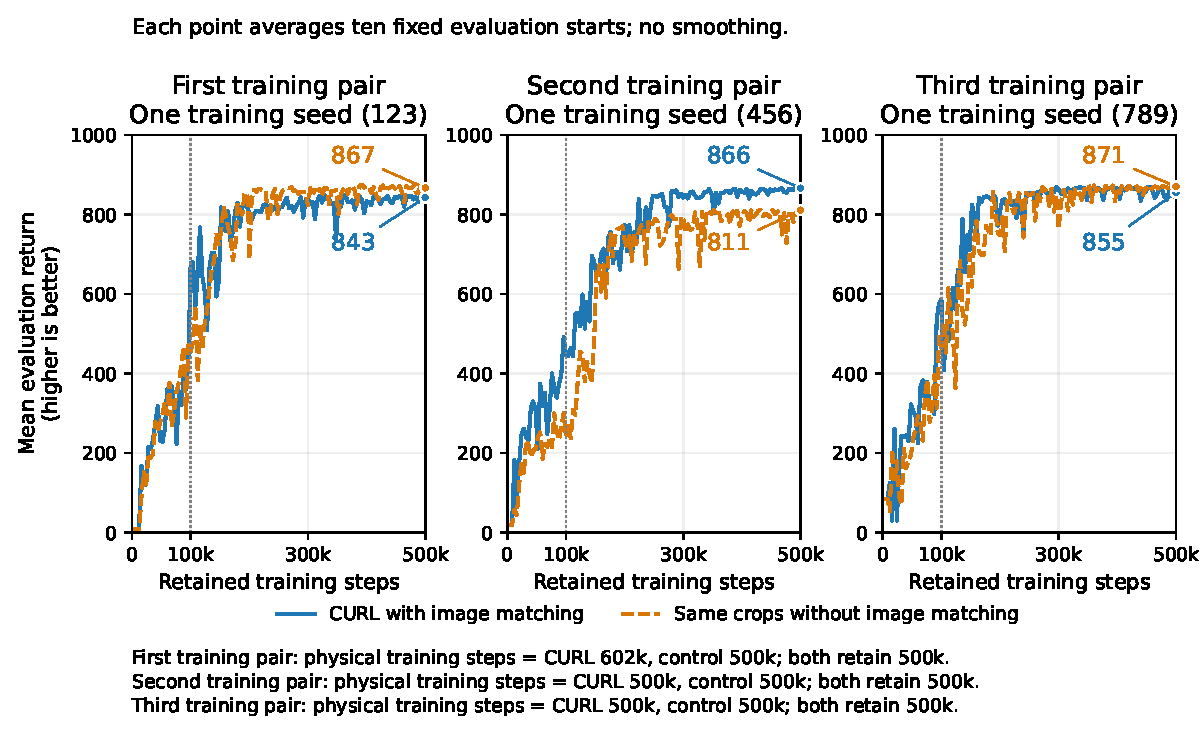
\includegraphics[width=.96\linewidth]{figures/three-completed-pairs/completed-500k-pairs.pdf}
\end{center}

Each panel is one training seed. Each line follows one model; each point averages
ten fixed evaluation episodes. Both methods use random image crops. Only CURL
has the extra image-matching exercise. Higher reward is better.

\question{What does this tell us?}

The control finished higher in two pairs; CURL finished higher in one. We see
an early benefit, but no consistent late winner in these three runs. Close
averages do not prove equivalence. We compare planned final checkpoints, not
the best point on each curve. Page 10 checks the early effect on a different task.

\question{A recovery cost matters when interpreting this plot.}

The first CURL model repeated 102,000 interactions after a save failure, using
602,000 in total. The other five models each used 500,000.
The axis shows retained training history, excluding the abandoned branch.
These plots do not establish an advantage at equal computing cost.

\takeaway{An extra learning exercise can help early without producing a clear final advantage. This small, one-task study motivates checking another task, not claiming a universal rule.}

\small
\textbf{Evidence.} Three completed pairs, training seeds 123, 456 and 789, on
\texttt{cartpole/swingup}. Native records and the dated paired summary are in
\texttt{extension-data/}. Evidence cutoff: 5 October, 00:46 UTC.
\end{frame}
\begin{frame}[t]
\vspace*{0.55in}
\chapterpage{9 / A SECOND TASK}{Does image matching help with walking?}

In \texttt{walker/walk}, a simulated body learns to stay upright and move forward
using pictures. We trained fresh models, not the cartpole models.

\begin{center}
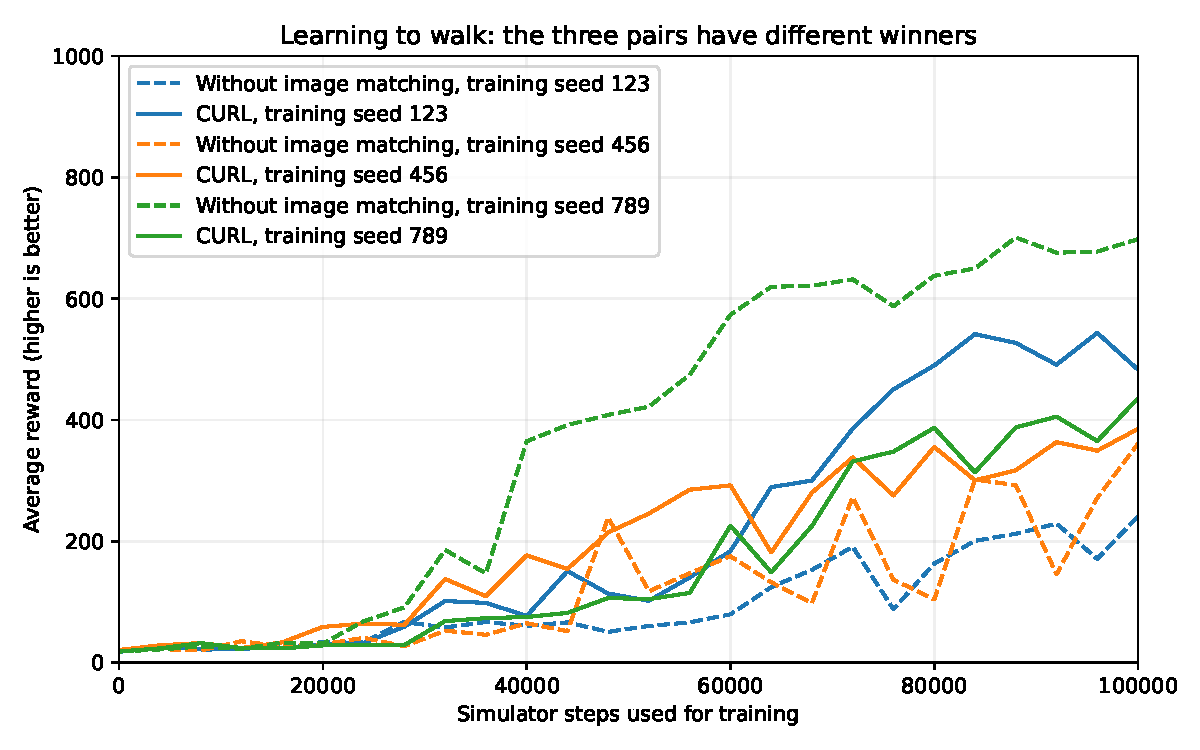
\includegraphics[width=\linewidth]{figures/walker-three-pairs/learning-curves.pdf}
\end{center}

\textbf{How to read the plot.} Each point averages ten test episodes without
changing the weights. Each color is one training pair. Solid lines include image
matching; dashed lines keep the crops but remove matching. Higher is better.

\question{Why is the average not enough?}

At the fixed 100,000-step endpoint, CURL scored \textbf{483 versus 241} for
the control, then \textbf{385 versus 361}, and \textbf{436 versus 698}.
CURL won twice; the control won the third by a large margin. Their average
scores, \textbf{435 and 433}, hide those different outcomes. We show every
curve without smoothing or choosing the best checkpoint.

\question{What can we conclude, and what comes next?}

Three pairs establish neither a dependable winner nor a tie. The next page
tests whether different starting states change this pattern.

\takeaway{Our question is not just whether a model learns. We want to know
which extra learning exercise helps, on which task, and how repeatable its benefit is.}

\small
\textbf{Cost and evidence.} Each run used 100k training and 260k evaluation steps.
CURL took 75--77 minutes, controls 69--72; equal experience is not equal
computation. Records: \texttt{walker-data/}. Cutoff: 5 October, 08:03 UTC.
\end{frame}
\begin{frame}[t]
\vspace*{0.55in}
\chapterpage{10 / CHECKING THE TEST}{Do different starting states change the result?}

Suppose one learned walker handles most initial postures well but often falls
from a particular posture. A test with only ten starts could give a misleading
impression of that model. We therefore tested \textbf{every final walking model
on the same 50 new starts}, without changing its weights.

\question{The same winners appeared again.}

The table shows CURL's score minus the control's score. Positive numbers favor
CURL; negative numbers favor the control. A score is the average total reward
per test episode. It measures walking behavior, not percentage correct.

\begin{center}
\begin{tabular}{lrr}
\toprule
Training pair & Original 10 starts & New 50 starts\\
\midrule
First pair & $+242$ & $+287$\\
Second pair & $+24$ & $+23$\\
Third pair & $-262$ & $-241$\\
\bottomrule
\end{tabular}
\end{center}

On the new starts, the third pair scored \textbf{429 for CURL versus 670 for
the control}. Its opposite result did not disappear with more testing.

\question{What did we learn?}

The mixed pattern is not explained away by replacing the original ten test
starts. It persists in the same trained models on this larger panel. That makes
variation between training runs important to investigate. It does not yet tell
us which part of training creates the differences, or how often CURL helps.

\question{Why train more models instead of just testing these again?}

Testing one learned walker 50 times still gives us only one learned walker.
The fifty-start panel contains the original three training pairs, not 300
independent training runs. We also trained three additional pairs from fresh
weights, with unchanged settings, to test variation between trained models.
The whole new group is now complete. The next page reports every pair rather
than selecting the models that support the more favorable story.

\takeaway{More tests of the same models and training more models answer
different questions. We need to keep those sources of variation separate.}

\small
\textbf{Scope and evidence.} This is the same walking task, not transfer to a
new task. We used every fixed 100k model, with no checkpoint selection or further
learning. The original scores remain unchanged. This supplemental check cost
300 test episodes, 300k simulator steps and about 45 minutes. Native records:
\texttt{walker-fresh-starts-data/}; details: \texttt{WALKER\_FRESH\_STARTS.md}.
Supplemental cutoff: 5 October, 08:48 UTC.
\end{frame}
\begin{frame}[t]
\vspace*{0.55in}
\chapterpage{11 / TRAINING NEW MODELS}{The new group favors CURL, but not in every pair.}

We trained three more walking pairs from fresh weights. Each pair uses a new
training seed, which changes initialization and training randomness. Both
methods keep the same task, crops, settings and fixed 100,000-step budget.

\begin{center}
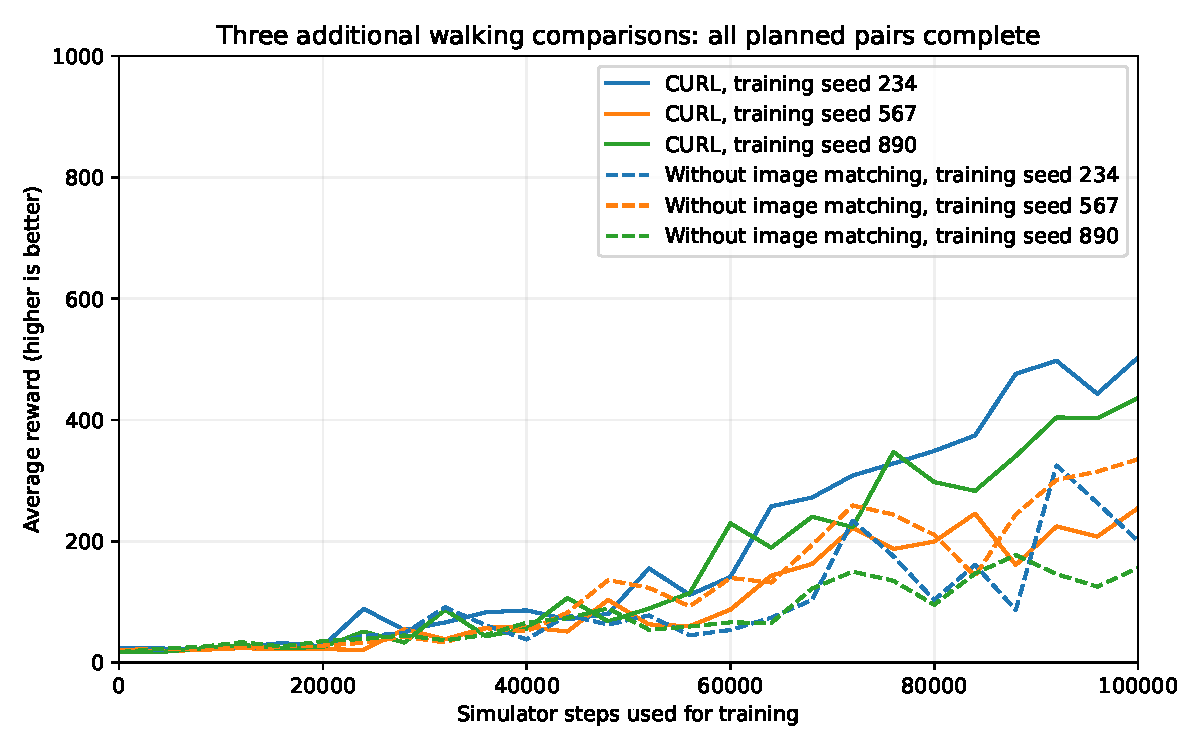
\includegraphics[width=.82\linewidth]{figures/walker-additional-three-pairs/learning-curves.pdf}
\end{center}

\textbf{Reading the plot.} Each color is a new training pair. Solid lines use
CURL; dashed lines remove image matching. Each point averages ten test episodes
without changing the model. Higher reward means better walking, not a success
percentage. All six curves are shown, without smoothing or checkpoint selection.

\question{What are the results at the planned endpoint?}

CURL scored \textbf{503 versus 200}, \textbf{255 versus 335}, and
\textbf{437 versus 156}. It won two pairs and lost one. This new group's
average is \textbf{398 versus 231}, an advantage of about 167 reward points.
The original group's average advantage was about 1 point. Both groups remain
in the report; neither replaces the other.

\question{What does this change?}

This adds positive evidence for CURL in this setting, while showing how much
the result can depend on training randomness. It does not establish a reliable
win on every run, an advantage on every task, or why the extra update helps.
The new group was added after inspecting the original results, so this remains
an exploratory study, not a new untouched confirmation.

\takeaway{A single average can hide important variation. Repeating the training
changed the size of the apparent benefit, but did not eliminate different winners.}

\small
\textbf{Evidence and cost.} All six runs finished without failures or restarts.
The group took 7.26 hours, including 3.53 hours of testing. Native records:
\texttt{walker-additional-data/}; figure and exact summary:
\texttt{figures/walker-additional-three-pairs/}. Cutoff: 5 October, 16:04 UTC.
\end{frame}
\begin{frame}[t]
\vspace*{0.55in}
\chapterpage{12 / CHANGING THE TEACHING TARGET}{Wrong image matches hurt learning here.}

Normally, two crops of the same recorded observation are the intended match.
We changed the exercise to treat another recorded moment as the match instead.
For example, a picture of the pole leaning right might be paired with one
from a different moment. This is a simplified example, not a saved image pair.
The reward-learning task and image crops stayed the same.

\begin{center}
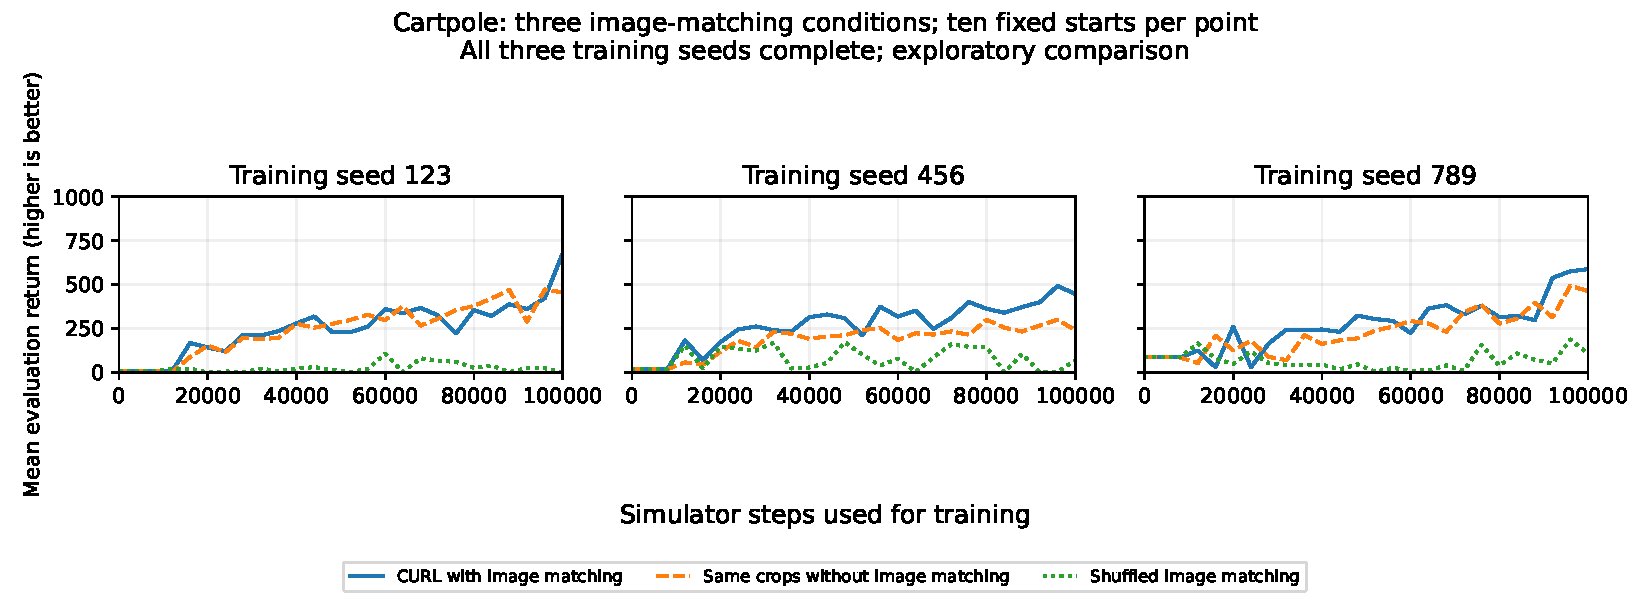
\includegraphics[width=.95\linewidth]{figures/correspondence-three-seeds/learning-curves.pdf}
\end{center}

Each panel shows one training seed. Blue uses correct matching, orange removes
the matching exercise, and green uses wrong matches. Each point averages ten
fixed test episodes. Reward measures swinging and balancing, not a percentage
correct. We compare every model at its planned 100,000-training-step checkpoint.

\begin{center}
\begin{tabular}{lrrr}
\toprule
Training seed & Correct matches & No matching & Wrong matches\\
\midrule
123 & 678.02 & 454.47 & 0.11\\
456 & 446.17 & 240.54 & 68.10\\
789 & 587.99 & 463.26 & 107.79\\
\bottomrule
\end{tabular}
\end{center}

\question{What does this show, and what does it not show?}

Wrong matching finished lower in all three comparisons. The average rewards
were \textbf{571, 386 and 59}, in the table's order. This is evidence that
incorrect teaching targets can damage learning in this setting. It is not
evidence that every model completely collapses, or that the same pattern holds
on other tasks.

\takeaway{A harmful teaching exercise is not a neutral control. Its poor result
does not, by itself, explain why correct matching helps. The next page tests
whether a smaller update changes the effect of both correct and wrong targets.}

\small
\textbf{Evidence.} Three new models from fresh weights, compared with the six
original cartpole models. No best-checkpoint selection; test episodes are not
extra training replicates. Native records: \texttt{correspondence-data/} and
\texttt{data/}; figure and exact summary: \texttt{figures/correspondence-three-seeds/}.
Cutoff: 5 October, 16:52 UTC. This is an exploratory follow-up, not a novelty claim.
\end{frame}
\begin{frame}[t]
\vspace*{0.55in}
\chapterpage{13 / CHANGING THE UPDATE}{A smaller update did not remove the harm.}

Could wrong image matches hurt mainly because the model changes too much
when learning from them? We repeated both the correct- and wrong-matching
conditions with a smaller update to the image encoder, the part that turns
pictures into useful features. Each model started from fresh weights.

\question{What exactly changed?}

The original code changes the encoder twice from the same matching-loss
gradient, using two separate optimizers. We skip only the dedicated encoder
optimizer's step. The other still changes the encoder and the comparison
between image features. Reward-learning updates, image crops and matching
labels stay the same. This is not a proven bug fix, and it does not halve all learning.

\question{Every result at the planned endpoint}

\begin{center}
\begin{tabular}{lrrr}
\toprule
Training condition & Seed 123 & Seed 456 & Seed 789\\
\midrule
Correct matches, original update & 678.02 & 446.17 & 587.99\\
Correct matches, smaller update & 795.84 & 316.12 & 531.20\\
\midrule
No matching exercise & 454.47 & 240.54 & 463.26\\
\midrule
Wrong matches, original update & 0.11 & 68.10 & 107.79\\
Wrong matches, smaller update & 138.08 & 72.01 & 19.90\\
\bottomrule
\end{tabular}
\end{center}

Each score averages total reward over ten fixed test starts after 100,000
cartpole training steps. Higher means better swinging and balancing, not
percentage correct. A seed changes initialization and training randomness;
each row contains three separately trained models. We use final checkpoints,
not the highest point on each learning curve.

\question{What did we learn?}

With correct matches, the smaller update helped once and hurt twice.
All three models still beat their no-matching comparison, but this change is
not consistently better than original CURL. With wrong matches, the scores
rose twice and fell once. All three still scored below no matching.

\takeaway{Wrong teaching targets remained harmful at both tested update
strengths. Making the update smaller was not a dependable rescue or a
consistent improvement. This is a limit on a proposed explanation, not
proof that update strength never matters.}

\question{Why did we repeat the comparison?}

Three seeds could not tell us how repeatable these differences were. We
therefore repeated both correct-matching rules and no matching on three new
seeds. Page 15 shows those results; no new wrong-target models were included.
Different policies collect different experience, so neither comparison
isolates an immediate encoder effect on identical data.

\small
\textbf{Evidence and cost.} The six new runs took 86.67 minutes, including
36.68 minutes testing and 38.71 seconds saving. No restarts or failures.
Native records: \texttt{encoder-strength-data/}, with original
comparisons in \texttt{data/} and \texttt{correspondence-data/}.
Details: \texttt{ENCODER\_UPDATE\_CONTROL.md}. Cutoff: 5 October, 18:18 UTC.
This adaptively chosen, one-task comparison is exploratory.
\end{frame}
\begin{frame}[t]
\vspace*{0.55in}
\chapterpage{14 / REPEATING THE COMPARISON}{The benefit did not repeat in every run.}

We repeated the comparison with three new training seeds: nine models in total.
A seed changes random initialization and training choices. Every model starts
from fresh weights, uses the same random-crop procedure, and receives 100,000
cartpole training steps. Both CURL versions use correct picture matches.

\begin{center}
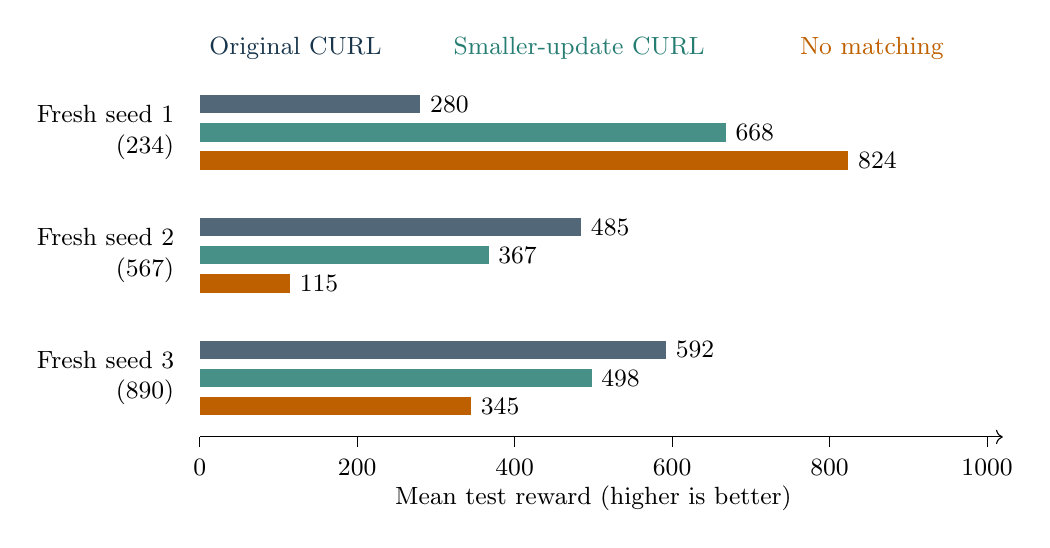
\begin{tikzpicture}[x=1cm,y=.65cm]
  \node[anchor=west,font=\small,text=ink] at (0,7.3) {Original CURL};
  \node[anchor=west,font=\small,text=accent] at (3.1,7.3) {Smaller-update CURL};
  \node[anchor=west,font=\small,text=orange!75!black] at (7.5,7.3) {No matching};
  \foreach \y/\v/\label/\shade in {
    6.2/2.8041343059/280/ink!75,
    5.65/6.6821960748/668/accent!85,
    5.1/8.2396888394/824/orange!75!black,
    3.8/4.8454970983/485/ink!75,
    3.25/3.6696917796/367/accent!85,
    2.7/1.1484934610/115/orange!75!black,
    1.4/5.9234426355/592/ink!75,
    .85/4.9773706413/498/accent!85,
    .3/3.4476950436/345/orange!75!black}{
    \fill[\shade] (0,\y-.18) rectangle (\v,\y+.18);
    \node[anchor=west,font=\small] at (\v,\y) {\label};
  }
  \node[anchor=east,align=right,font=\small] at (-.2,5.65) {Fresh seed 1\\(234)};
  \node[anchor=east,align=right,font=\small] at (-.2,3.25) {Fresh seed 2\\(567)};
  \node[anchor=east,align=right,font=\small] at (-.2,.85) {Fresh seed 3\\(890)};
  \draw[->] (0,-.3)--(10.2,-.3);
  \foreach \x/\label in {0/0,2/200,4/400,6/600,8/800,10/1000}{
    \draw (\x,-.3)--(\x,-.5);
    \node[anchor=north,font=\small] at (\x,-.55) {\label};
  }
  \node[font=\small] at (5,-1.5) {Mean test reward (higher is better)};
\end{tikzpicture}
\end{center}

Each bar is \textbf{one trained model}, tested on the same ten fixed starts.
The score is mean total reward for swinging and balancing the pole, not
percentage correct. We use final checkpoints, not the best point on each curve.

\question{What repeated, and what changed?}

In the original three seeds, both matching methods always beat no matching.
In this new group, both won twice and lost once. The smaller update improved
on original CURL once and worsened it twice, as it did in the original group.

\takeaway{Repeating the comparison changed the conclusion: matching helped
in every original seed, but not every new seed. The benefit depends on the
training run.}

\question{Why not just report the averages?}

The averages are 452 for original CURL, 511 for the smaller update and 428
for no matching. The smaller update's one large gain over original CURL
outweighs two losses. Yet no matching did better still on that first seed.
Three seeds do not establish a dependable winner.

\question{What is the next useful question?}

Does matching improve the model's visual features, or mainly change which
experiences it collects while learning? A proposed follow-up would give both
update rules the same saved experience. That could isolate an immediate update
effect, but would not by itself show better control. It has not been run yet.

\small
\textbf{Evidence.} Nine completed runs; no restarts or failures.
Records: \texttt{fresh-seed-data/}; protocol: \texttt{CARTPOLE\_FRESH\_SEEDS.md}.
Reviewed: 7 October, 08:45 UTC. This added group is exploratory, chosen after
earlier results and reported separately. No novelty claim is made.
\end{frame}
\end{document}
